\section{Anhang}
\label{sec:Anhang}
\subsection{Technische Daten}
\begin{table}[H]
    \centering
    \caption{Technische Daten der Dopplerflüssigkeit.}
    \label{tab:Daten_Dopplerflüssigkeit}
    \begin{tblr}{colspec={c c}}
        \toprule
        Dichte & $\rho = 1,15\,\unit[per-mode=fraction]{\gram\per\cubic\centi\meter}$ \\
        Schallgeschwindigkeit & $c_{\text{L}}=1800\,\unit[per-mode=fraction]{\meter\per\second}$\\
        Viskosität & $\eta = 12\,\unit{\milli\pascal\second}$ \\
        \bottomrule
    \end{tblr}
\end{table}
\begin{table}[H]
    \centering
    \caption{Technische Daten des Dopplerprisma.}
    \label{tab:Daten_Dopplerprisma}
    \begin{tblr}{colspec={c c}}
        \toprule
        Schallgeschwindigkeit & $c_{\text{P}}=2700\,\unit[per-mode=fraction]{\meter\per\second}$\\
        Länge & $l = 30,7\,\unit{\milli\meter}$ \\
        \bottomrule
    \end{tblr}
\end{table}
\begin{table}[H]
    \centering
    \caption{Technische Daten der Strömungsrohre.}
    \label{tab:Daten_Rohre}
    \begin{tblr}{colspec={c c}}
        \toprule
        Innendurchmesser & Außendurchmesser\\
        \midrule
        $7\,\unit{\milli\meter}$ & $10\,\unit{\milli\meter}$ \\
        $10\,\unit{\milli\meter}$ & $15\,\unit{\milli\meter}$\\
        $16\,\unit{\milli\meter}$& $20\,\unit{\milli\meter}$\\
        \bottomrule
    \end{tblr}
  \end{table}

\subsection{Originaldaten}
%
\begin{figure}[H]
  \centering
  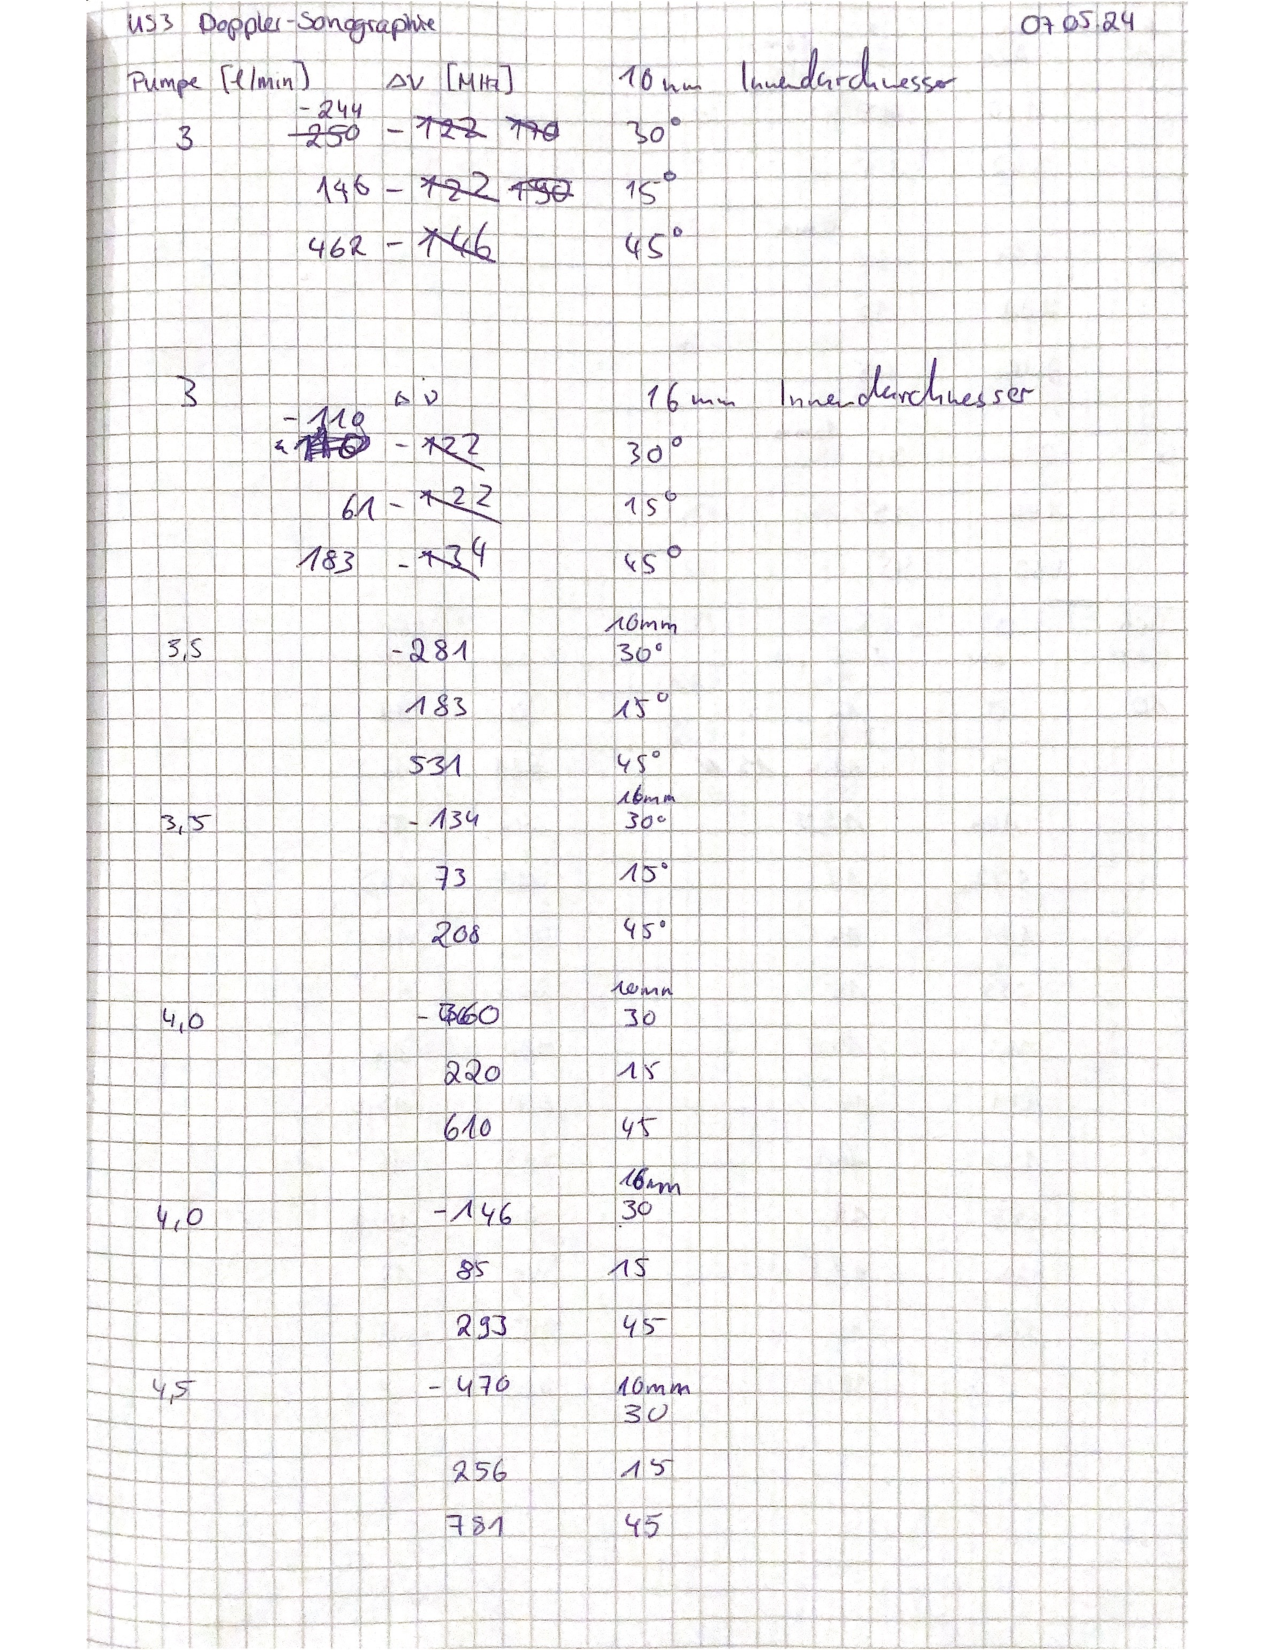
\includegraphics[width=0.9\textwidth]{content/Messdaten/US3_1.pdf}
  \label{fig:Messungen_1}
\end{figure}
\begin{figure}[H]
  \centering
  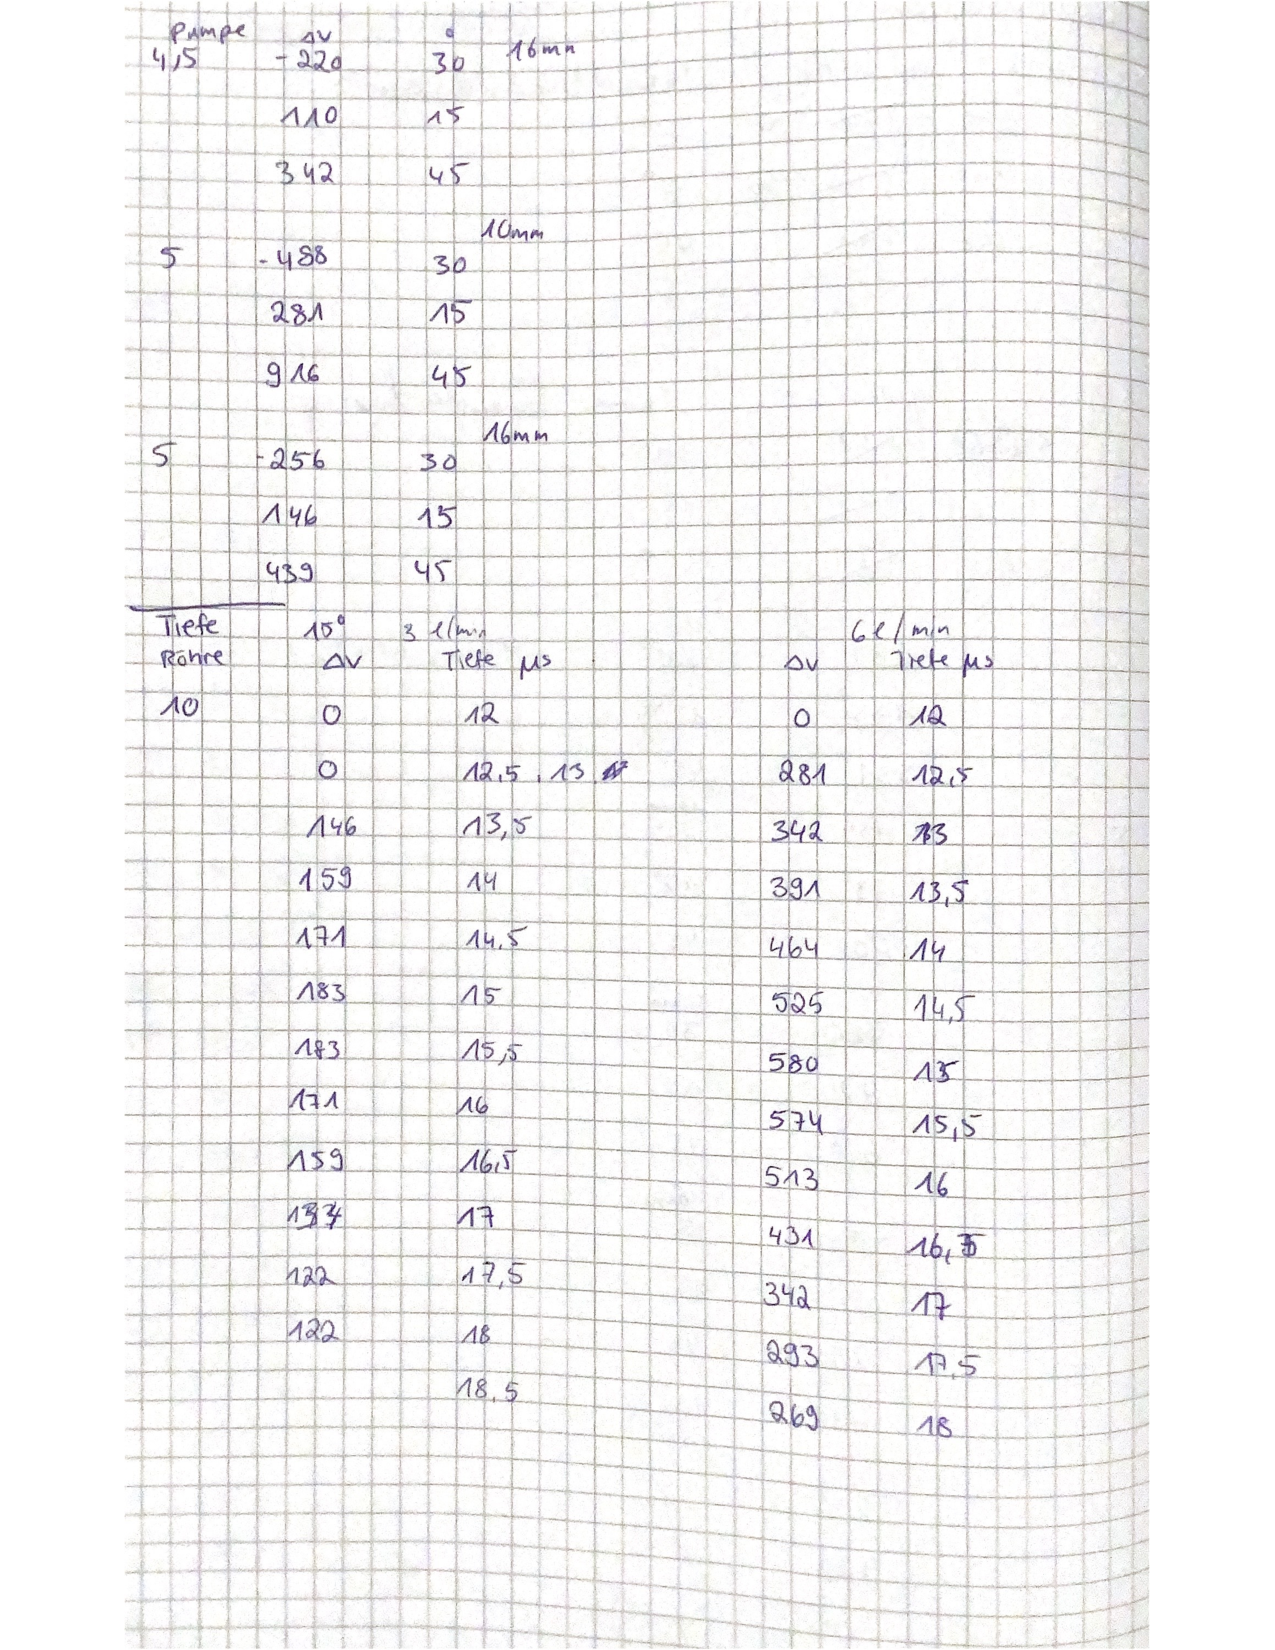
\includegraphics[width=\textwidth]{content/Messdaten/US3_2.pdf}
  \label{fig:Messungen_2}
\end{figure}
\begin{figure}[H]
  \centering
  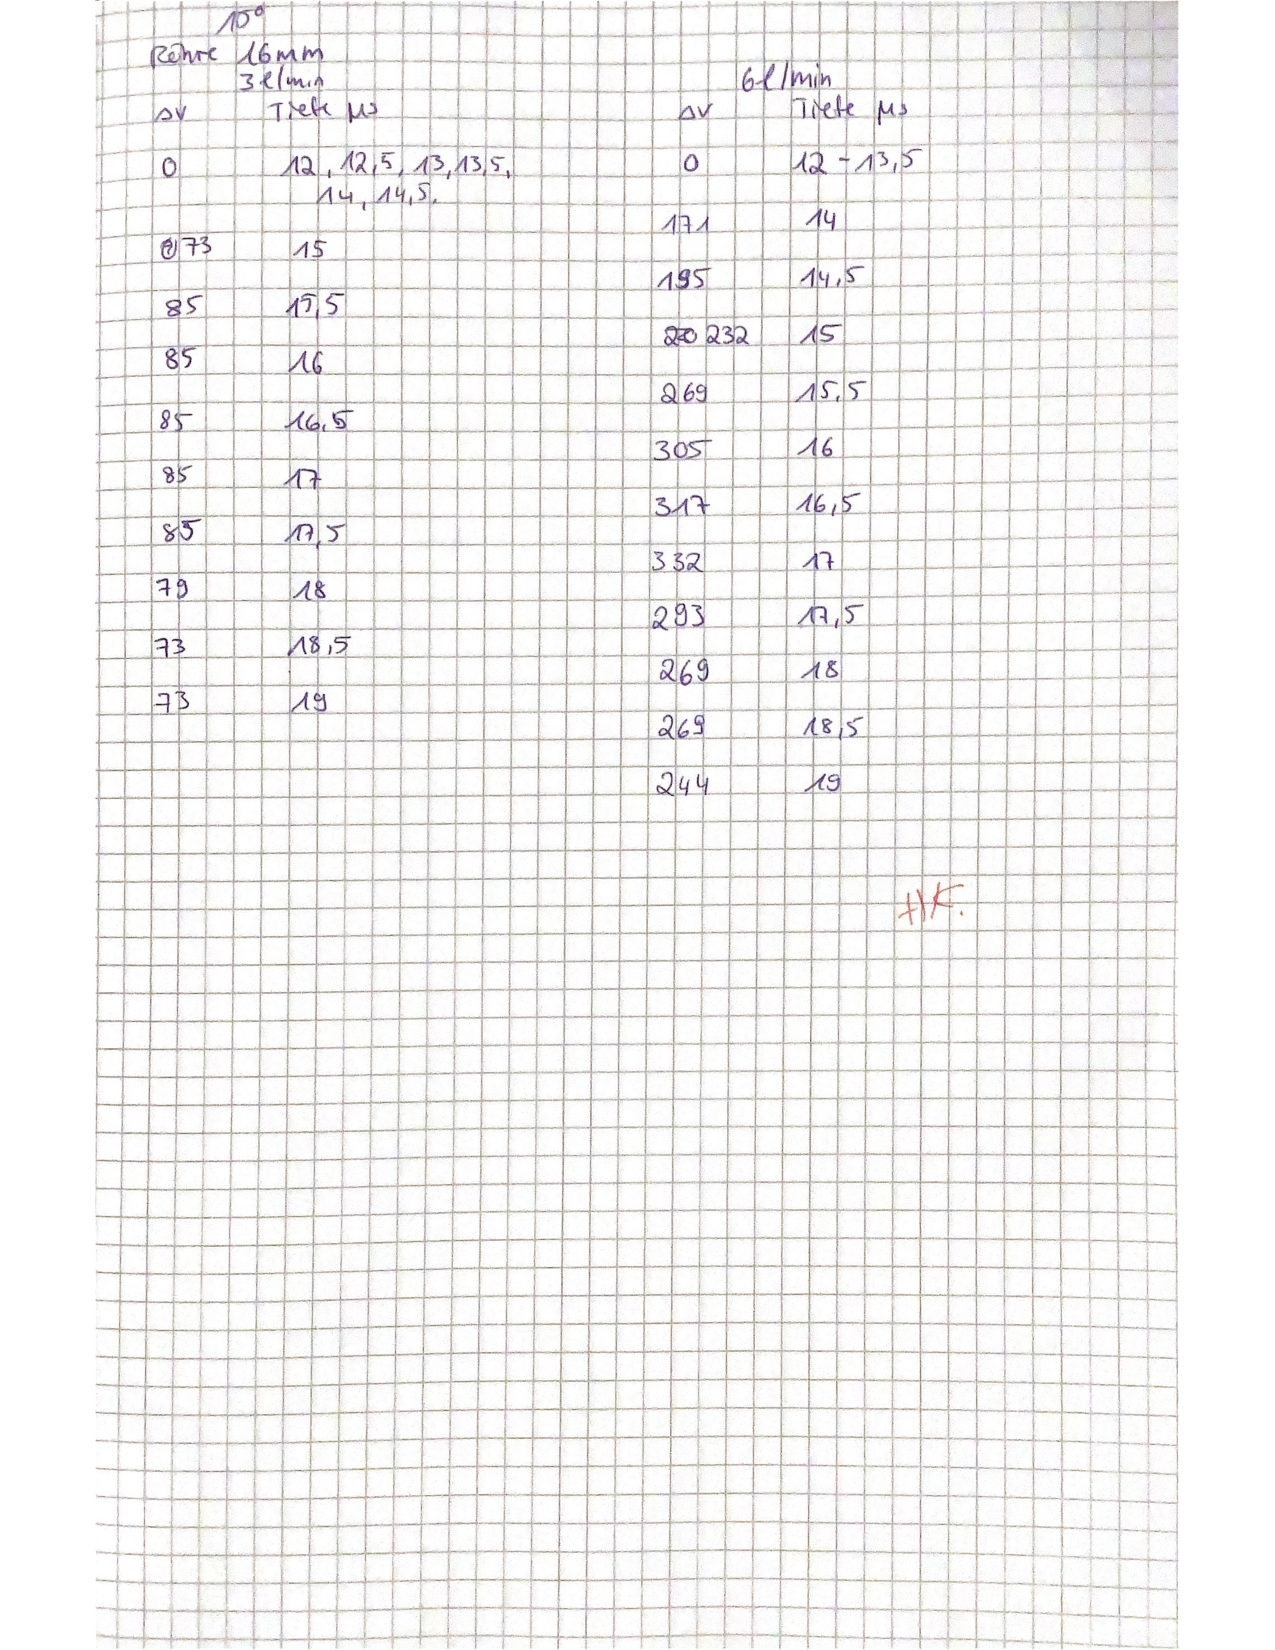
\includegraphics[width=\textwidth]{content/Messdaten/US3_3.pdf}
  \label{fig:Messungen_3}
\end{figure}